\section{Introduction}



Additive manufacturing (or 3D Printing) is an emerging technology, in which
different objects are printed in layers having a 3D model as a reference. This technology made rapid prototyping faster and enabled the creation of custom-shaped objects. However this process is not always perfect and printing errors are to be expected. Manually reviewing every print job is a tedious labor work and naturally the desire of automatization of anomaly detection rose. \\
One interesting 3D printing technique, sand 3D printing, stands out by not using any heat. This allows printing objects of very large sizes, but comes with a specific type of printing defects: scratches. \\
In this thesis a YOLO-based neural network solution is proposed and analyzed for this automatization procedure. \\
TODO: motivation
TODO: one abstraction layer above

TODO: insert example of scratch


\subsection{Printing process}
The 3D printer in the experiments at hand is sand based, more specifically binder jetting technology. With this technology, a layer is printed by laying a powder bed, then the printer applies drops of binding agent in regions of the bed to bond the powder particles together \cite{binder_jetting}. For each layer a bitmask is provided, which shows the regions that need to be printed. \\
In order to better track the printing process, the 3D printer has an internal camera that captures each printed layer. The captured images are then calibrated. In figure \ref{fig:layer_bitmask} a printed layer and the respective bitmask can be seen.\\
In our case the printing errors are scratches on the printed surfaces like in figure \ref{fig:layer_00325_marked_cropped}.


\begin{figure}[ht]
  \centering

  \begin{subfigure}{\textwidth}
    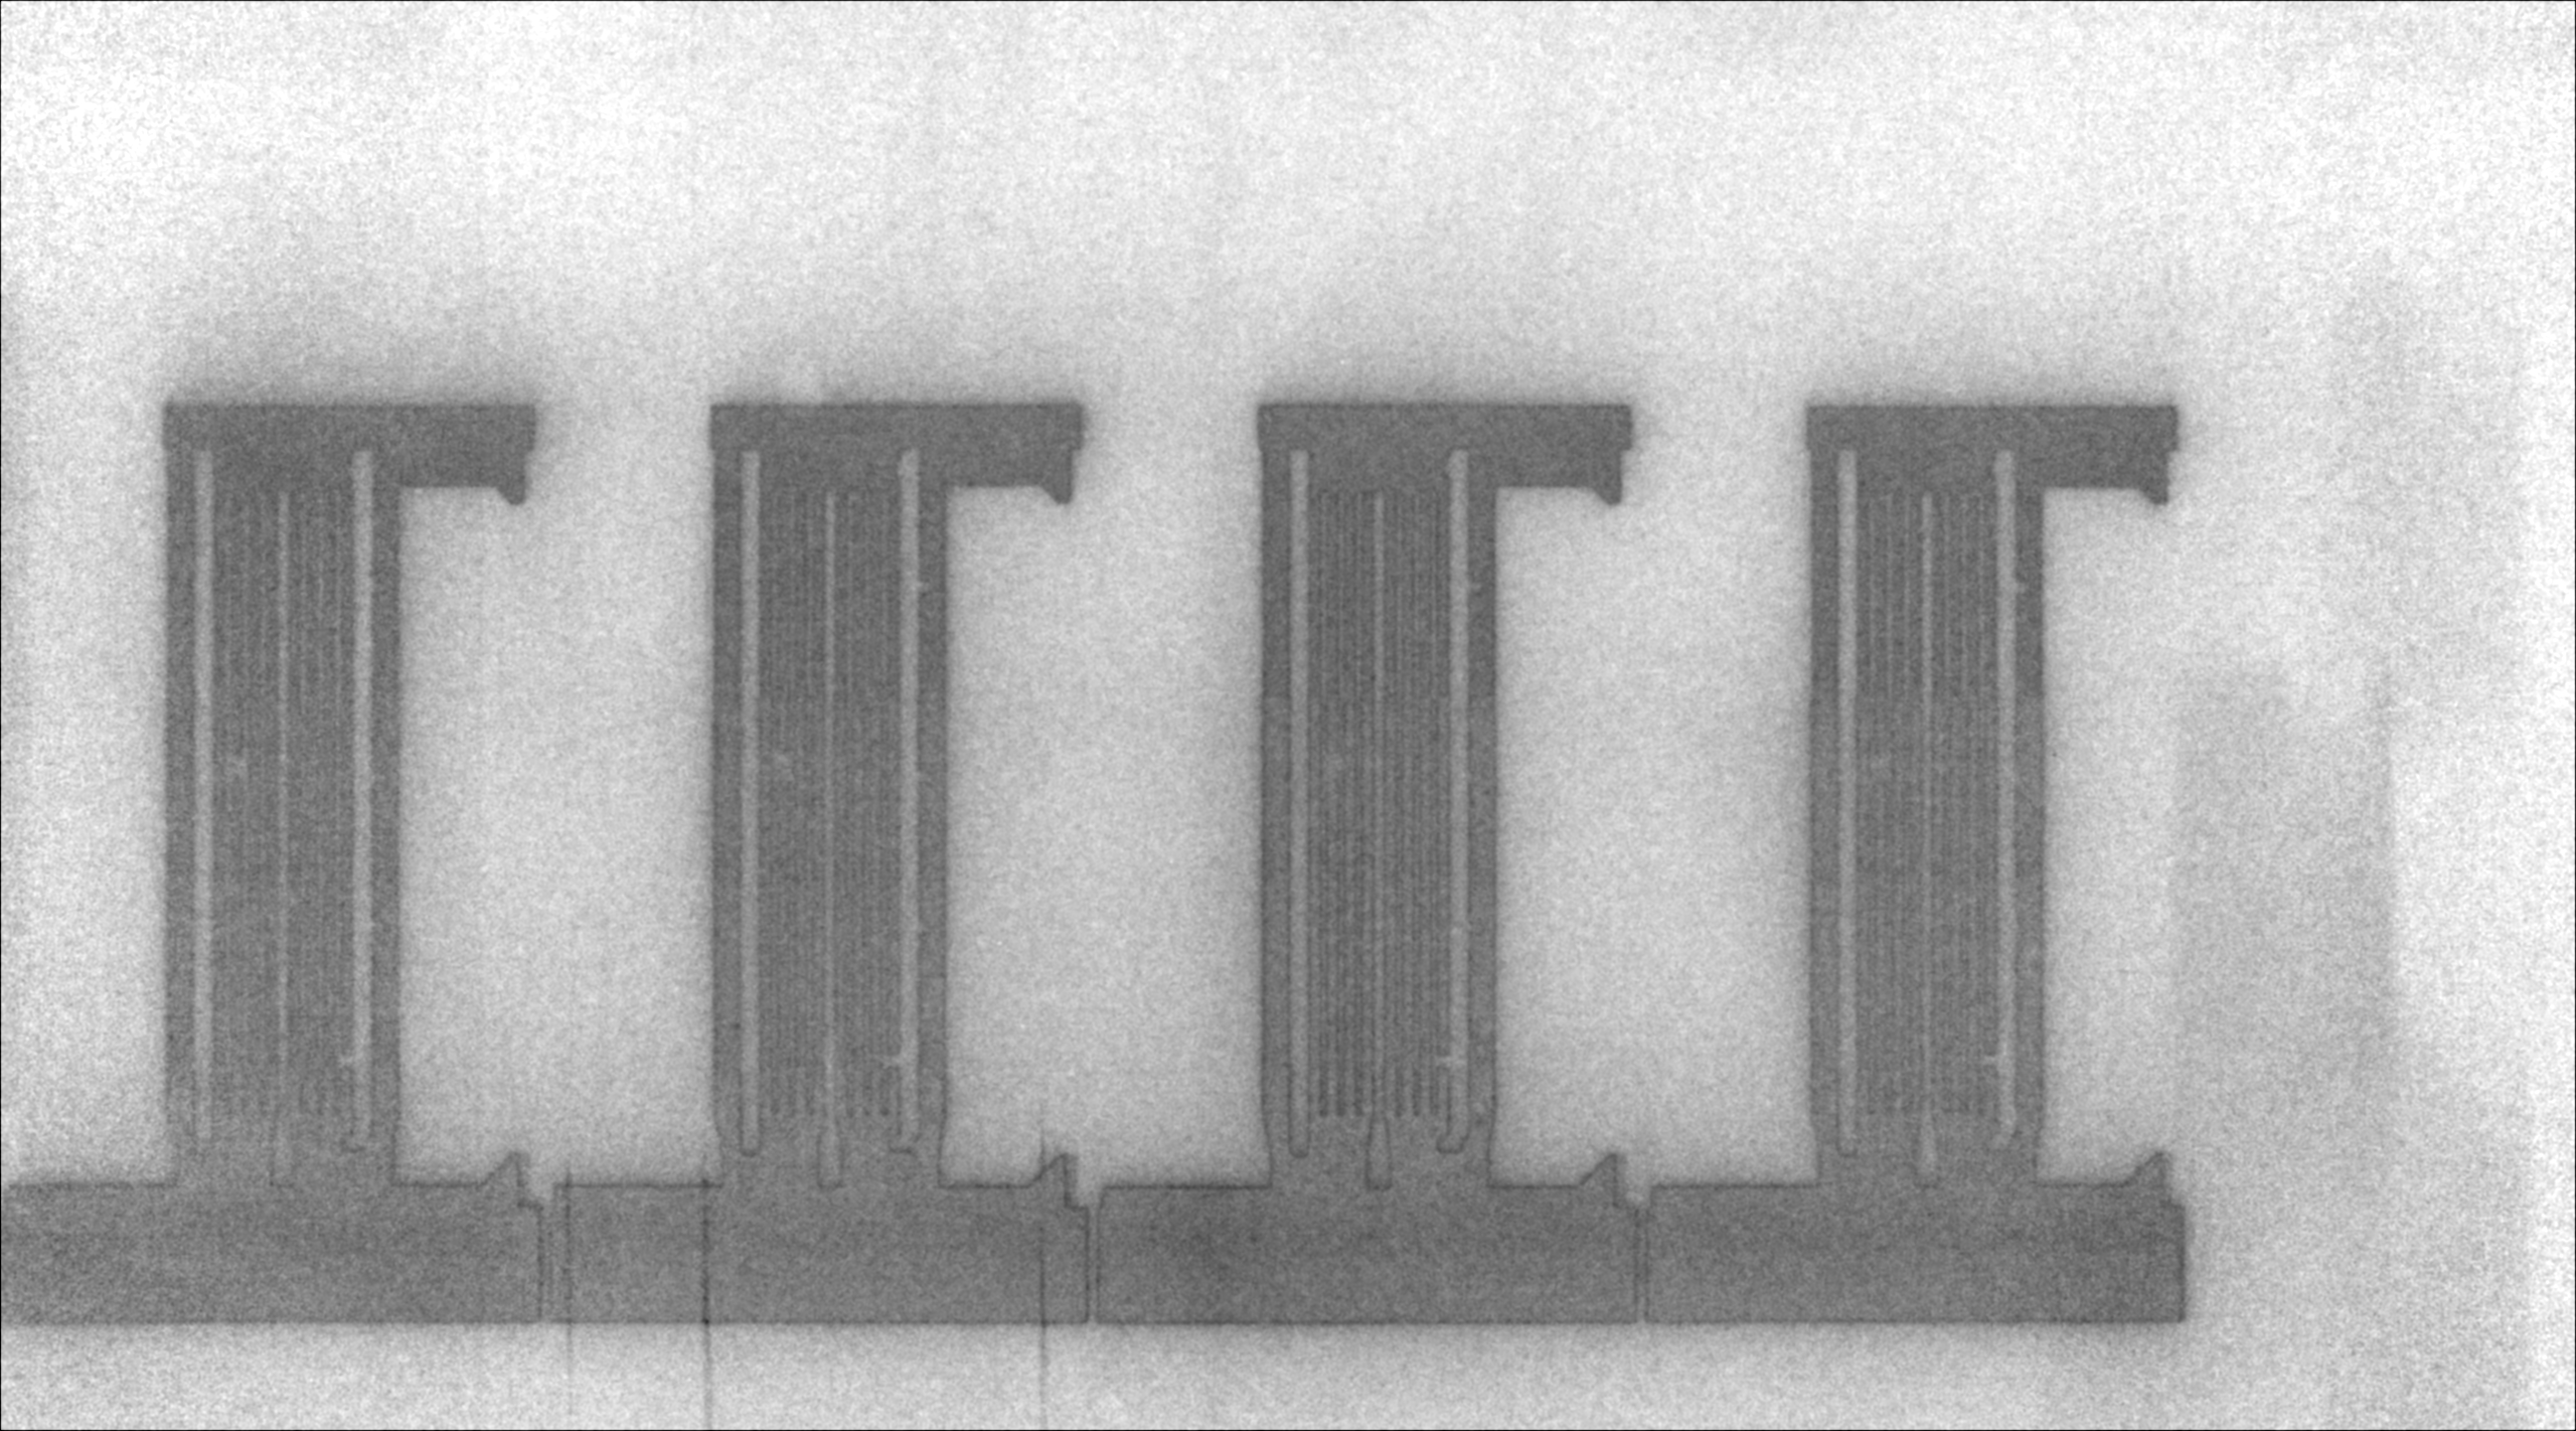
\includegraphics[width=\textwidth]{images/layer_00325}
    \caption{Calibrated capture of a layer.}
    \label{fig:layer}
  \end{subfigure}

  \begin{subfigure}{\textwidth}
    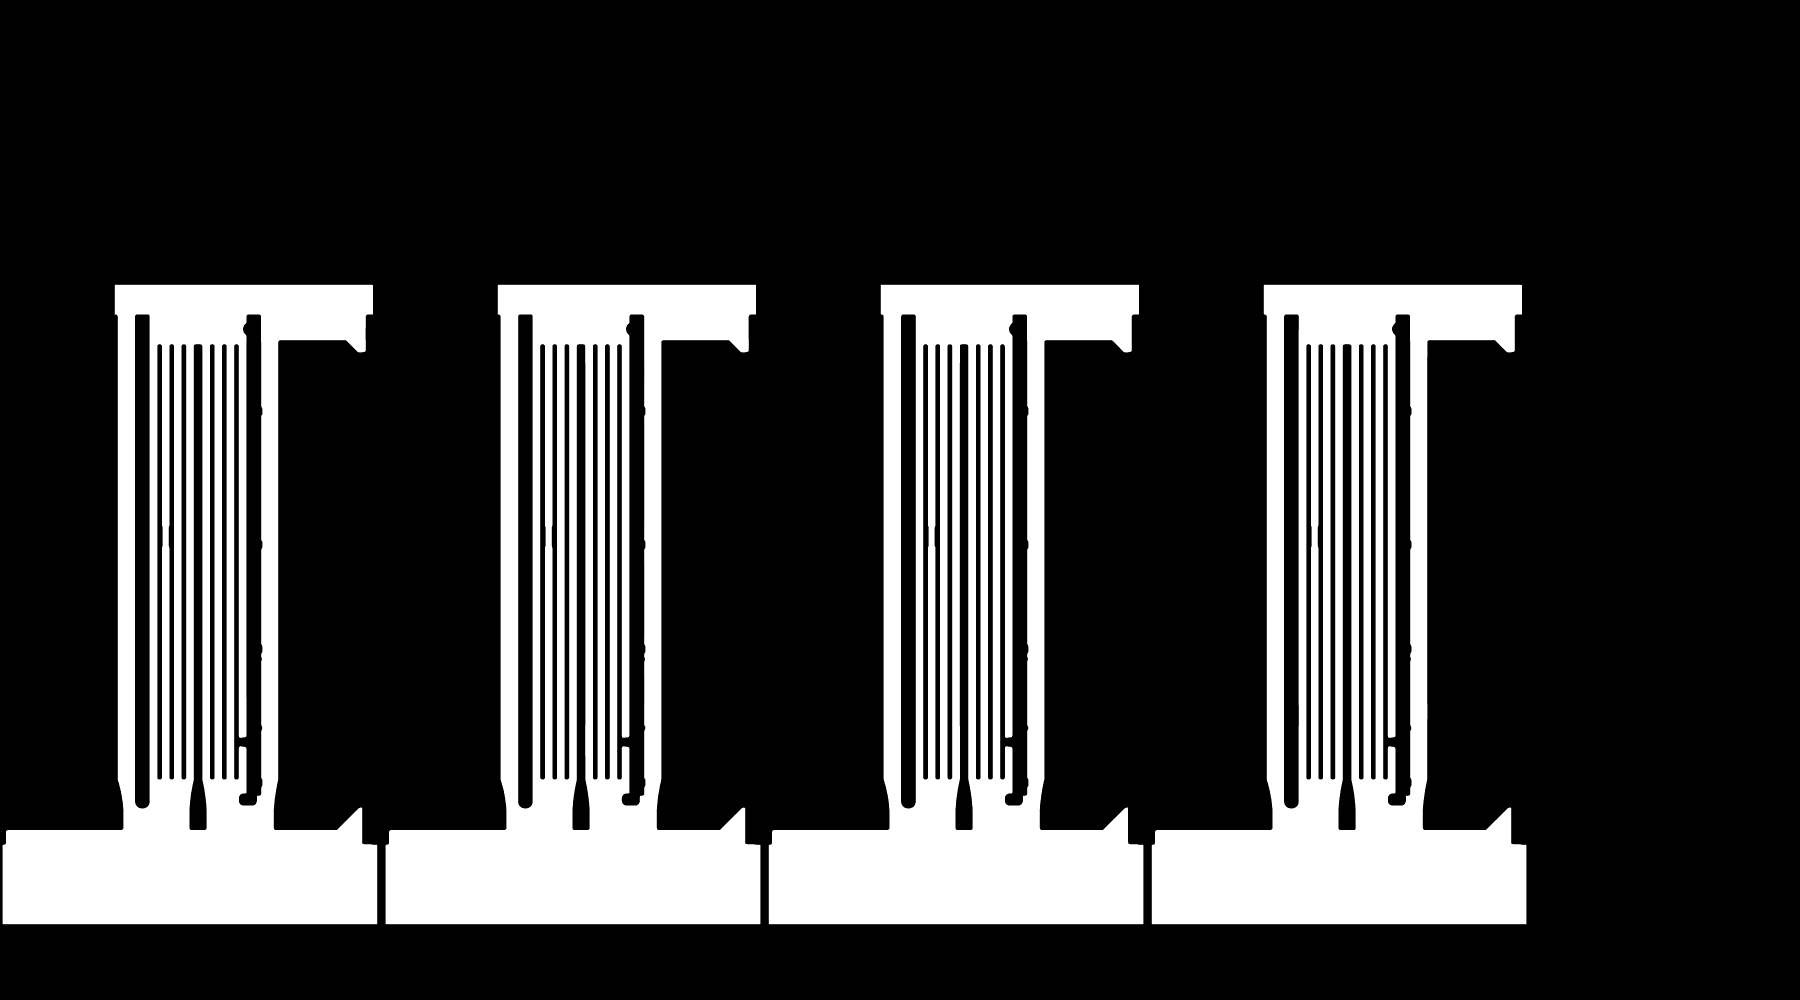
\includegraphics[width=\textwidth]{images/bitmask_00325}
    \caption{Bitmask used by 3D Printer as layer model.}
  \end{subfigure}

  \caption{Printed layer with the respective bitmask.}
  \label{fig:layer_bitmask}

\end{figure}


\begin{figure}[ht]
  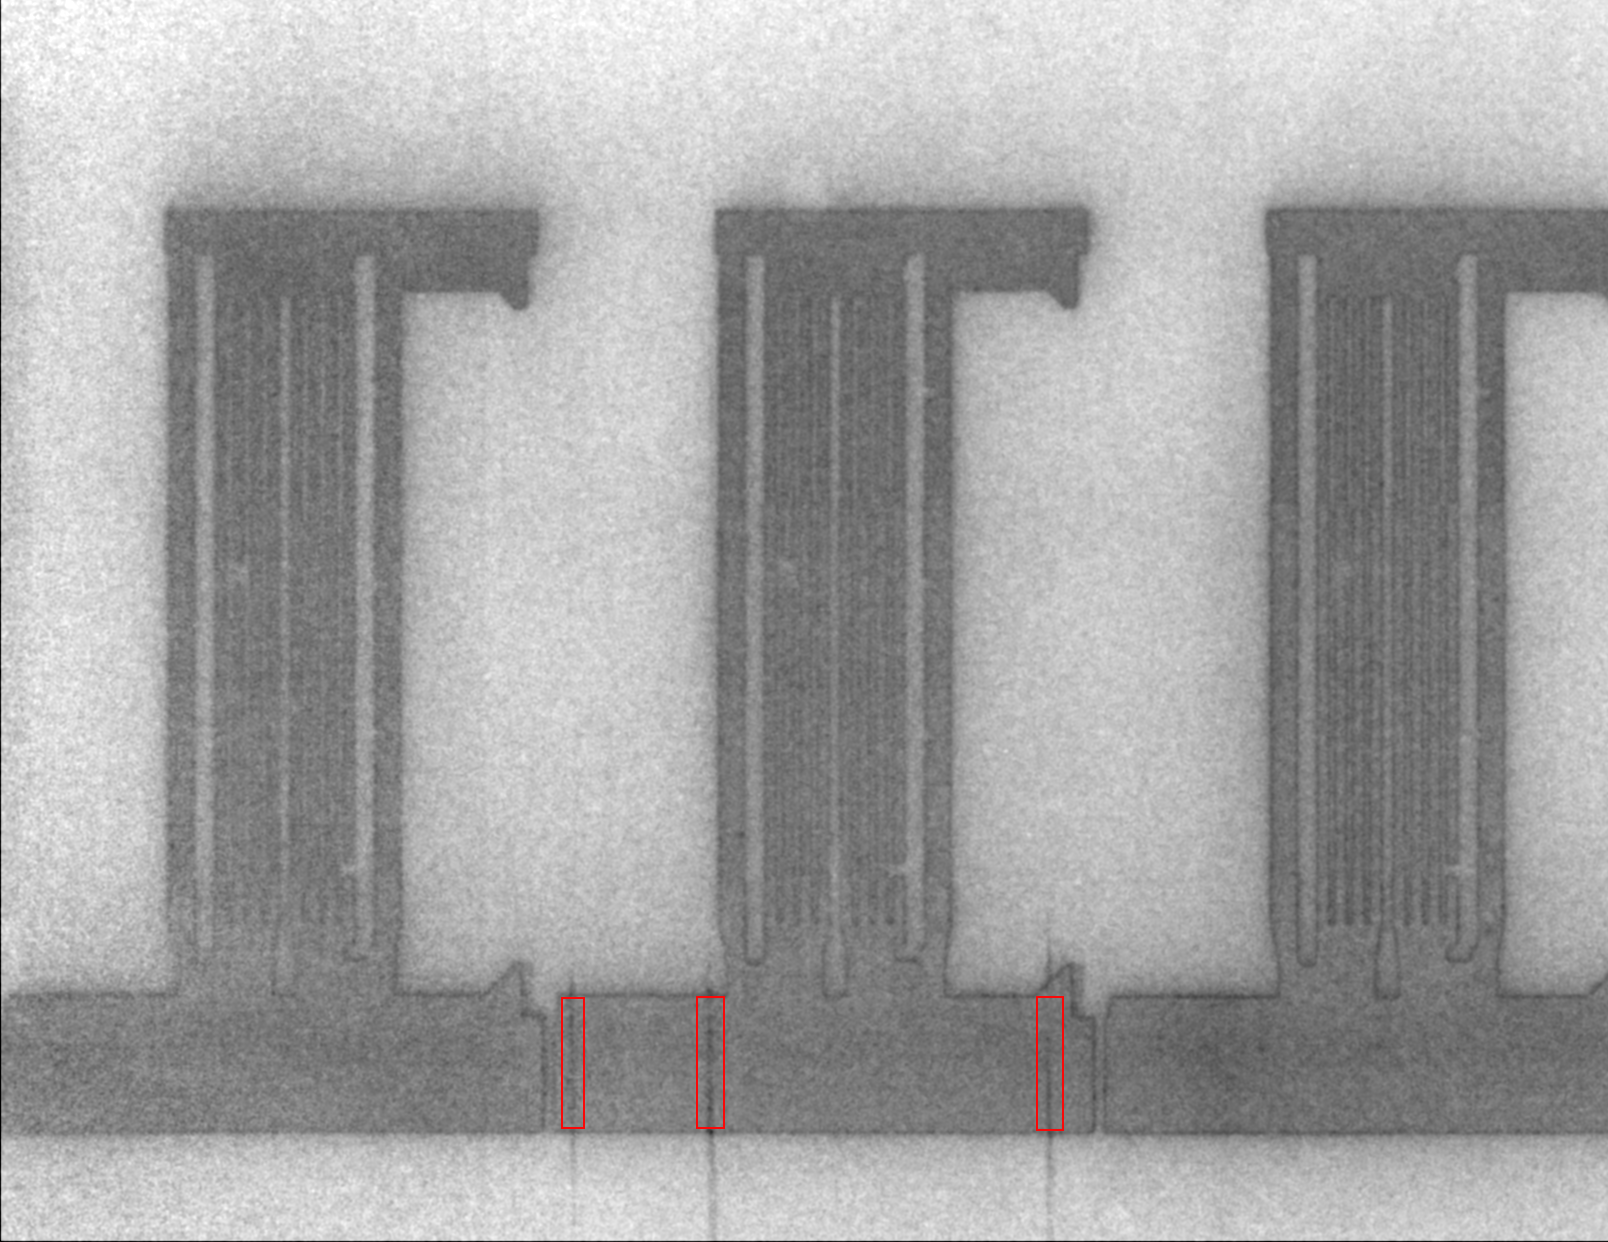
\includegraphics[width=0.65\textwidth]{images/layer_00325_marked_cropped}
  \centering
  \caption{Scratches marked from figure \ref{fig:layer}}
  \label{fig:layer_00325_marked_cropped}
\end{figure}

TODO: OD with NN, bb and semantic segmentation, vezi bookmark nou
\subsection{Object Detection (With Neural Networks)}
There are a variety of techniques used to perform object detection. Initially, object detection was posed as a non-neural computer vision problem, but this required a constant and tedious manual tuning of parameters. In order to avoid this tuning, feature-based machine learning algorithms were developed e.g. Viola-Jones algorithm \cite{viola_joines_paper}. In this way the parameter tuning was partially automatized, but it still required manual tuning like selecting optimal the window size and appropiate Haar features for the Viola-Jones algorithm.
One step further in this direction was the introduction of deep-learning based methods, which use a neural network at heart. A trained neural network would be albe to detect objects with way less parameter tuning. The drawback is that a considerable amount of labeled data for training is now required, which mostly is manually labeled. Luckily, today there are many open source labeled datasets that easily contain hundreds of thounsands of images e.g. ImageNet Dataset \cite{imagenet_site}, OpenImages Dataset \cite{openimages_site}. \\
Because of the already labeled datasets, the manual labor for deep-learning based methods was greatly reduced and the focus shifted towards those kind of methods, leading to the creation of many innovative models. One distinction among deep-learning based methods, regarding data labeling, is that the objects can be labeled with bounding boxes or segmentation masks. Models that use bounding boxes tend to train and predict faster, while models with segmentation masks will have the benefit of optimizing predictions to a pixel level. Another consideration would be that, if manual labeling is required, drawing bounding boxes is easier and less error prone than drawing an outline for segmentation masks. \\

\begin{figure}[!h]
\centering
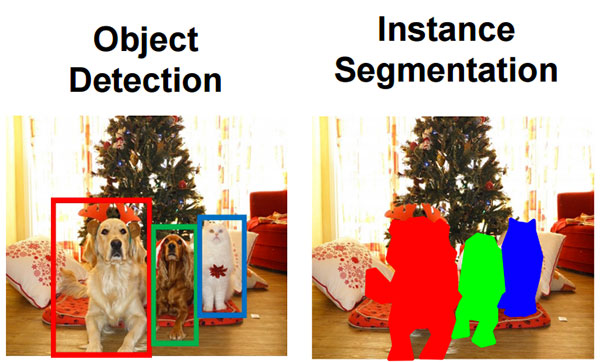
\includegraphics[width=0.65\textwidth]{images/bbs_vs_seg}
\caption{Labeling methods: on the left bounding boxes, on the right segmentation masks}
\end{figure}

Regarding the architecture of neural networks, the detection process may have one or two stages. In a single stage network the prediction is made directly from the extracted features of the image, while in a two stage network the network proposes some regions in the first stage and in the second stage the proposed regions are classified. Initially, single stage detectors predicted faster and could be used for real-time detections, but where performing poorer than two-stage detectors. Conversely, two-stage detectors were not optimal for real-time detection, but were more precise. This rule of thumb got overwritten with the release of You Only Look Once object detector (YOLO).

\begin{figure}[!h]
\centering
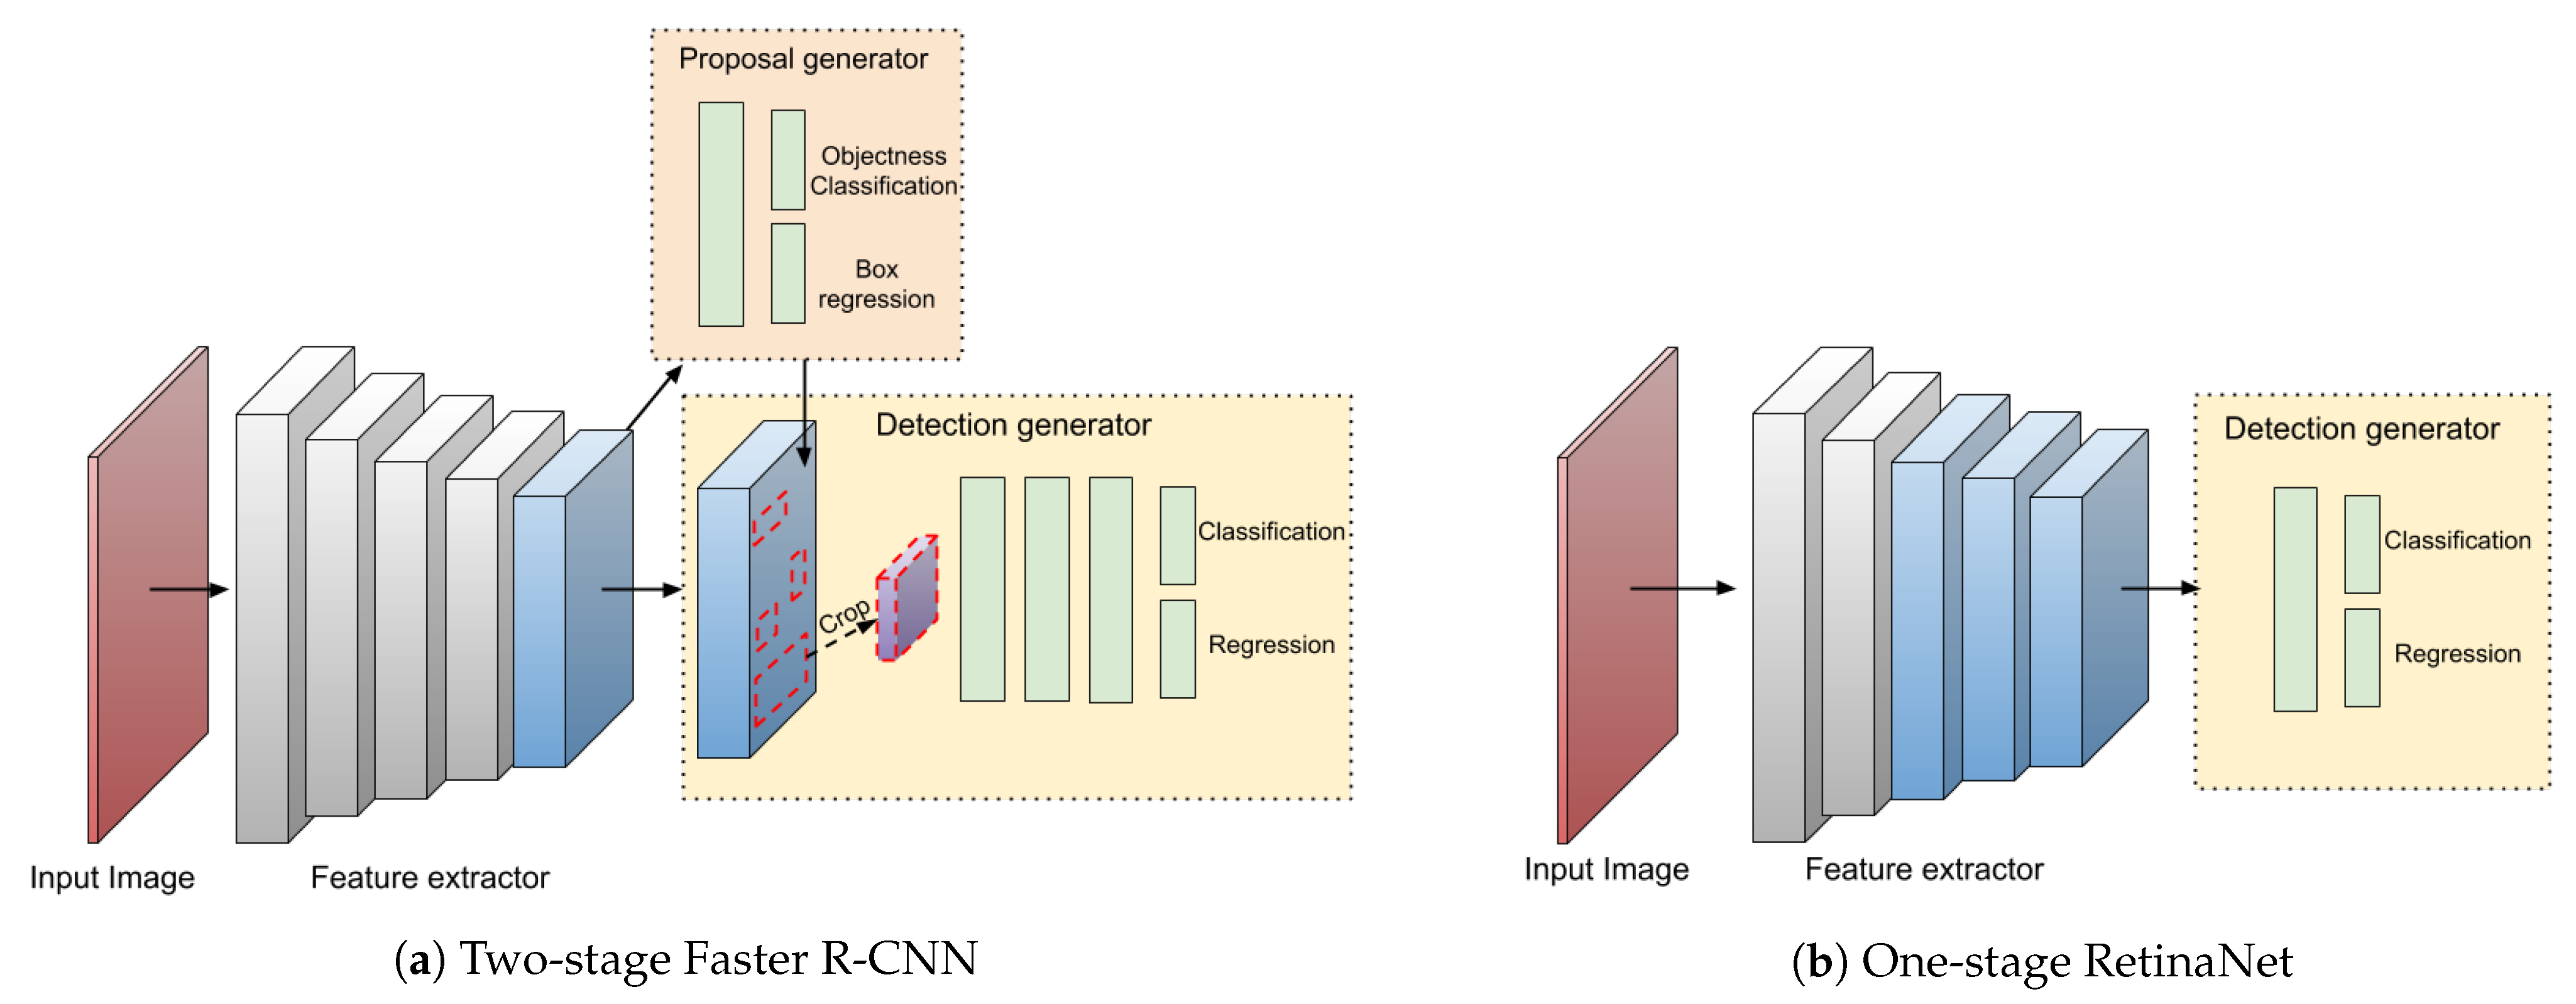
\includegraphics[width=0.75\textwidth]{images/single_stage_vs_two_stage}
\caption{Comparing stage types of object detectors.}
\end{figure}



The first YOLO object detector, now known as YOLOv1 \cite{yolov1_paper}, got a lot of attention for outperforming the then state-of-the-art object detectors such as DPM \cite{dpm_paper}, Fast R-CNN \cite{fast_rcnn_paper} and Faster R-CNN \cite{faster_rcnn_paper}. Also the simplicity of YOLO was quite refreshing for using only 24 convolutional layers and 2 fully connected layers only, unlike the sophisticated R-CNN based architectures. \\
Even if in some very deep model variations of Fast and Faster R-CNN the mean average precision (mAP) was slightly better,the FPS counter would take a massive hit e.g. 0.5 FPS only for Fast R-CNN. \\

\begin{figure}[!h]
  \centering
  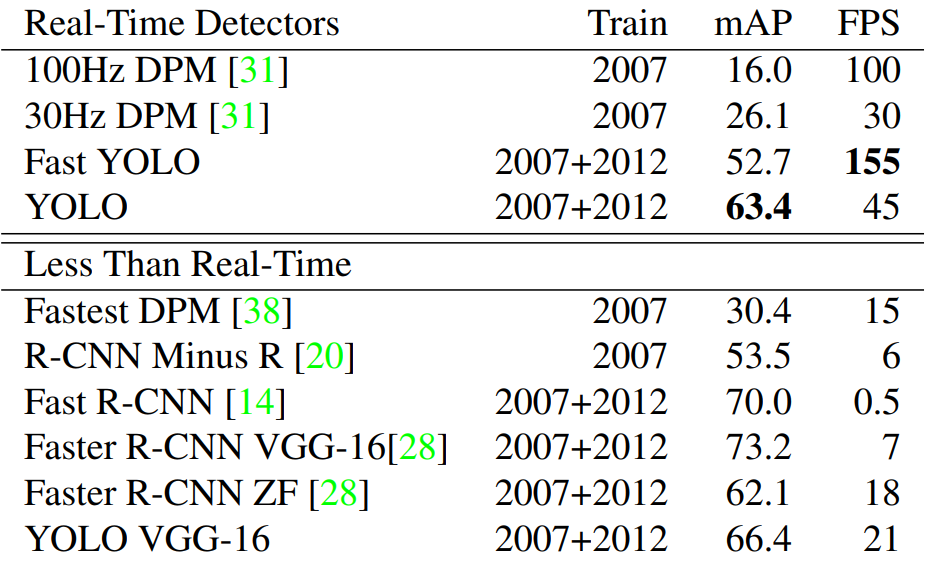
\includegraphics[width=0.75\linewidth]{images/yolo_images/compare_yolov1}
  \caption{TODO: make own table. YOLOv1 compared to then state-of-the-art models \cite{yolov1_paper}}
\end{figure}


This first successful initial release of YOLO was a launch pad for development of subsequent YOLO versions, so that a new class of object detectors was born. This class of architecture contains 3 main components: backbone, neck and head.
The backbone has the role to extract features from the image, while the neck tries to aggregate the features from different stages from the backbone. In the end the head does the prediction. Usually the backbone has a quite simple build like ResNet-101 and Darknet-53 \cite{yolov3_paper}.For feature aggregation SPP \cite{spp_paper} and FPN \cite{fpn_paper} are a popular choice . \\
Later on, different research groups developed their own YOLO-based object detectors and non-canonical versions like YOLOv5 \cite{yolov5_git} and YOLOR \cite{yolor_paper} were created. With this many releases from different research groups, simply taking the latest YOLO version was not a viable choice anymore and for this thesis multiple versions have been tests.\\

TODO: maybe talk about YOLO style labels



\iffalse
TODO: State of the art: RCNN, SSD, YOLO, EfficientDet(compound scaling)? \\
Meanwhile, there are multiple versions of YOLO \cite{yolov4_paper, yolov5_git, yolov7_paper}, but some of them are not canonical versions that are developed by the original authors. One such version is YOLOv5. From a performance point of view, YOLOv5 was performing better than YOLOv4, the latest fully developed canonical version \cite{yolov7_paper}, and it had a better design from a deployment and development point of view: written in PyTorch, supports Tensorboard visualization, better documentation. \\
YOLOv1-5 labels are bounding boxes with class id represented by 1 integer followed by 4 floats. The integer is the class id, the first 2 floats are the coordinates of the center of the bounding box and the next 2 floats are the width and height of the bounding box. The coordinates and sizes of the bounding box are normalized with respect to the image size. Additionally, an extra float can be used to represent confidence for detected bounding boxes.
The
\fi

\subsection{Main Challenges}
A first challenge was choosing the right YOLO version. As mentioned in the previous subsection, there are currently a multitude of YOLO versions developed by different research groups. The final decision was to use YOLOv5 by ultralytics \cite{yolov5_git} since it quickly displayed a good performance, was written in a popular framework like PyTorch and provided support for logging and debugging tools. Other versions, such as YOLOv4 \cite{yolov4_paper}, YOLOX \cite{yolox_paper} and YOLOR \cite{yolor_paper}, were some interesting candidates, but each came with it's drawbacks. YOLOv4 had similar performance to YOLOv5, however it had longer training times and a very rudimentary logging system (no support for tools like Tensorboard). YOLOR and YOLOX had interesting twists regarding the architectures, but YOLOX used a custom framework called MegEngine \cite{megengine_git} and YOLOR lacked documentation and large community support. A few initial experiments were also not better than YOLOR or YOLOX. \\
The small dataset is itself another challenge. The dataset contains only 2300 images, which is far less than the reference datasets like COCO \cite{coco_site} used for training and benchmarking object detecors, which contains over 300,000 images. \\
Another challenge is the domain knowledge integration. As explained at the beginning of this section, the printer uses a bitmask as a printing plan for each layer. This means, that an ideal reference image of the layer is available and this fact should be used, especially since the dataset is so small. However the problem is that the layer image capture by camera contains also segments and artifacts from the previous layer too. TODO WHY?. Therefore, the model must be aware of previous layers. \\


\iffalse
A prerequisite for best training results on YOLOv5 detectors is a large enough dataset with consistent labels and image variety \cite{yolov5_train_tips}. In the general case, this a trivial part, since there are many open source labeled datasets, like the COCO dataset \cite{coco}. In our case, the printing errors are not common objects that can be found in such datasets, so we need to create our own dataset and there are some challenges regarding this step.\\
TODO: Dark spots and fine scratches as one challenge: labeling scratches
\textbf{Dark spots:} Printindetectorsg a layer is not an instant process and the ??oxidation?? of layers is sometimes uneven, therefore the light is reflected at different strengths along the printed region. As a consequence, the camera might capture some dark marks that are hard to determine if they are scratches as seen in figure \ref{fig:layer_dark_scratch}.\\
\textbf{Fine scratches:} Not all scratches are equal, making some of them barely visible and from an practical point of view they might be irrelevant. A metric is required for a consistent labeling. \textit{TODO: vielleicht einen Beispiel?}\\
\textbf{Small number of samples:} YOLO based detectors require usually at least 10 000 instances per class, but in our case we have only TODO instances.
\fi

\begin{figure}[ht]
  \centering

  \begin{subfigure}{\textwidth}
    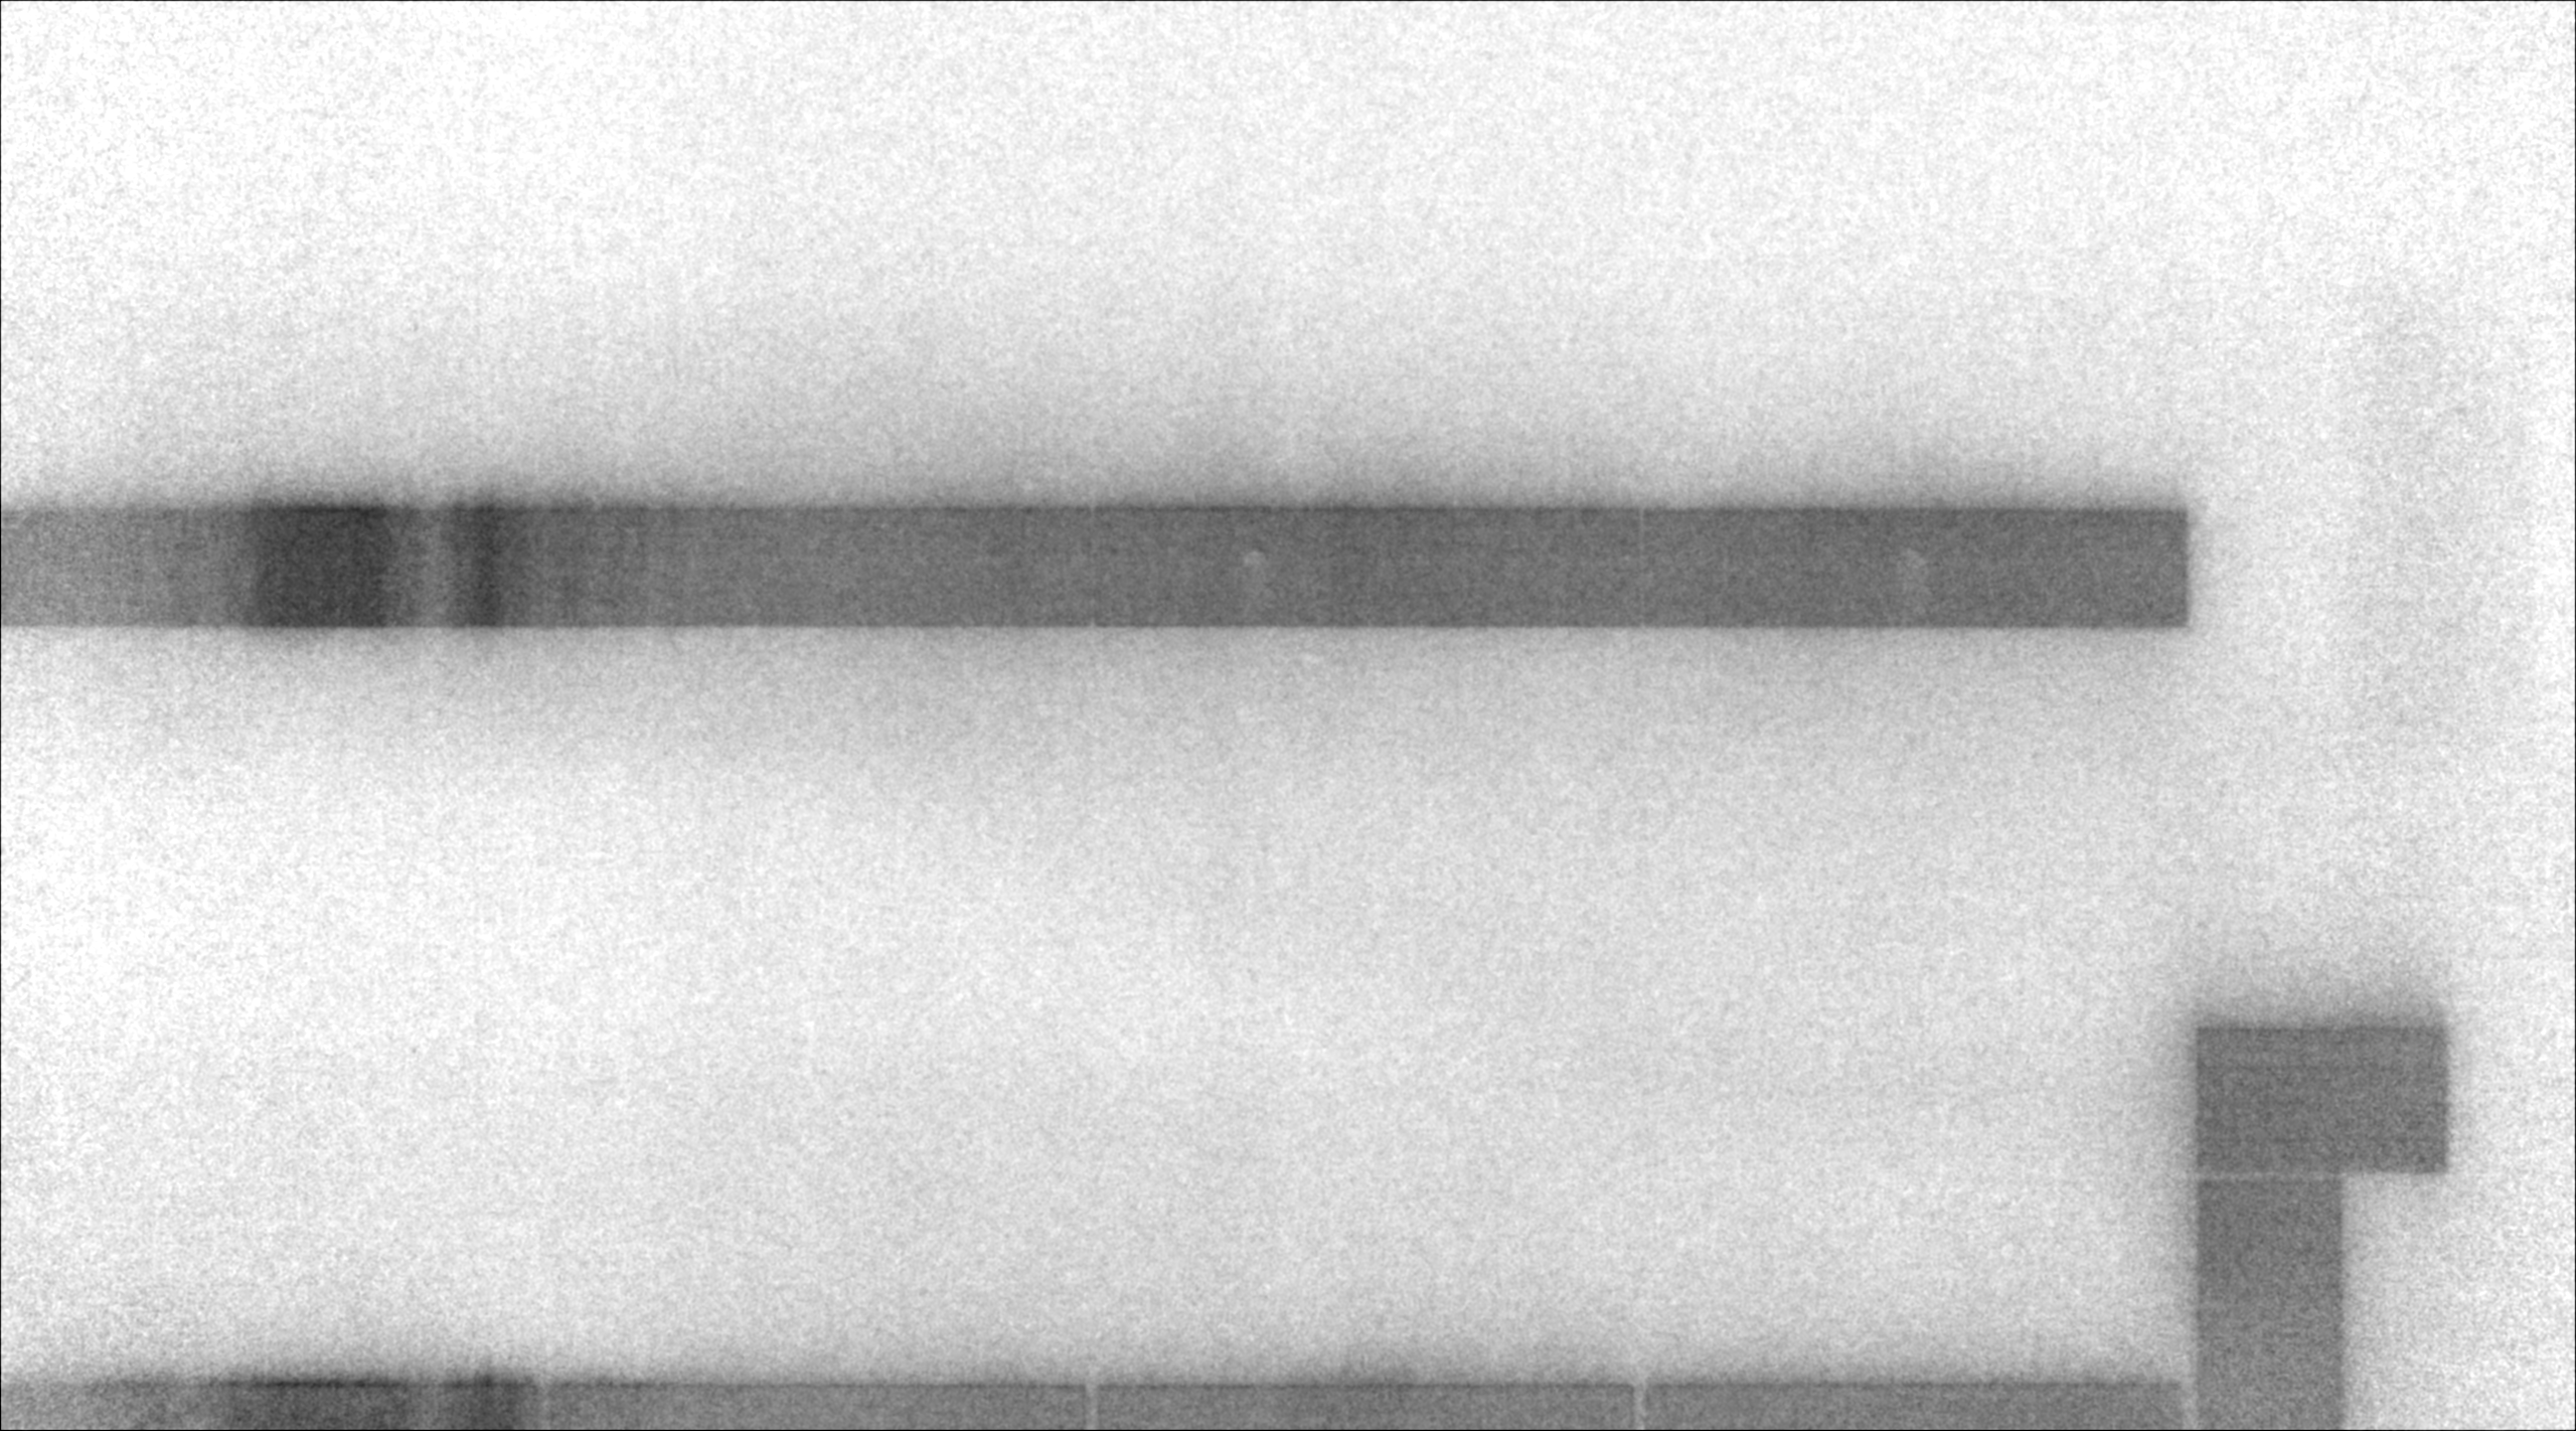
\includegraphics[width=\textwidth]{images/layer_dark_scratch}
    \caption{Layer with dark spots.}

  \end{subfigure}

  \begin{subfigure}{\textwidth}
    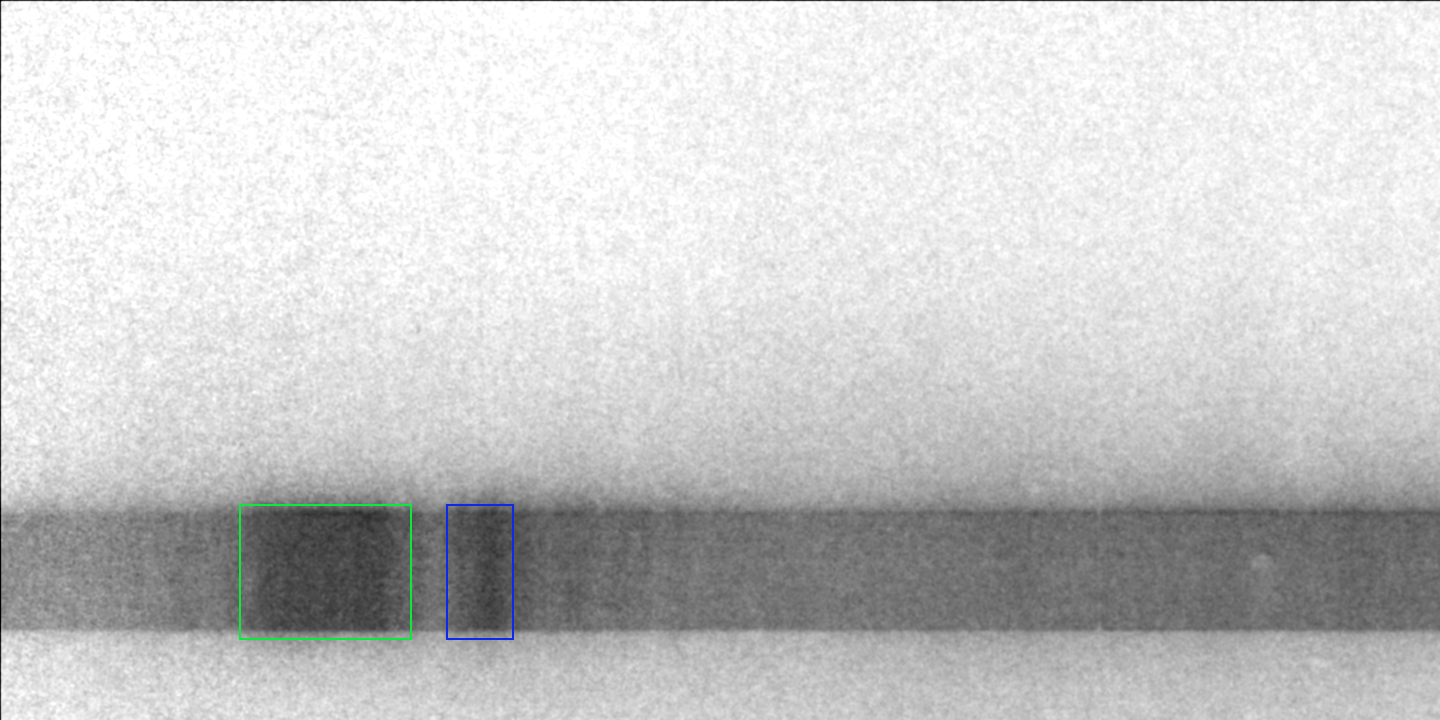
\includegraphics[width=\textwidth]{images/layer_dark_scratch_cropped}
    \caption{Zoomed to the upper left corner of the layer. The green bounding box is safely a dark spot, but the blue bounding box is an ambiguous case.}
  \end{subfigure}

  \caption{Dark spot or scratch?}
  \label{fig:layer_dark_scratch}


\end{figure}

\iffalse
\begin{verbatim}

Links:

URL list from Tuesday, Jul. 19 2022 22:06 PM
To copy this list, type [Ctrl] A, then type [Ctrl] C.

202112_proposal_thesis_AM.pdf
file:///home/captain/Downloads/202112_proposal_thesis_AM.pdf

additive manufacturing - Google Search
https://www.google.com/search?q=additive+manufacturing&oq=additive+manufacturi&aqs=chrome.0.69i59j69i57j0i512l2j0i20i263i512j46i512j69i60l2.3570j0j7&sourceid=chrome&ie=UTF-8

AM Basics - Additive Manufacturing (AM)
https://additivemanufacturing.com/basics/

Additive manufacturing, explained | MIT Sloan
https://mitsloan.mit.edu/ideas-made-to-matter/additive-manufacturing-explained

What is Additive Manufacturing? Definition, Types and Processes - TWI
https://www.twi-global.com/technical-knowledge/faqs/what-is-additive-manufacturing

What is Additive Manufacturing | GE Additive
https://www.ge.com/additive/additive-manufacturing

\end{verbatim}
\fi
